\documentclass[11pt]{article}
\usepackage[a4paper,margin=25mm]{geometry}
\usepackage[T1]{fontenc}
\usepackage[utf8]{inputenc}
\usepackage{lmodern,microtype,amsmath,amssymb,amsthm,booktabs,graphicx,natbib}
\usepackage[colorlinks=true,allcolors=blue,breaklinks=true]{hyperref}
\usepackage{url,placeins}
\newtheorem{proposition}{Proposition}
\newcommand{\E}{\mathbb{E}}
\newcommand{\R}{\mathbb{R}}
\newcommand{\norm}[1]{\left\lVert #1\right\rVert}
\title{Budget-aware reliability auditing of DFT force datasets\\[3pt]
\large Physical consistency, error prediction and missed failures}
\author{Sinan G\"okmen\\Department of Chemistry, Istanbul Technical University\\
\texttt{gokmens23@itu.edu.tr}}
\date{11 September 2026}
\begin{document}
\maketitle
\begin{abstract}
Large density-functional-theory datasets support molecular and materials discovery,
but the reliability of individual calculations remains a separate question from
surrogate-model accuracy. We formulate reliability auditing as a budgeted search
for discrepancies between existing force labels and tightly recomputed references.
Physical consistency scores and learned error predictors are compared with explicit
accounting for the reference calculations used to train the latter. A retrospective
benchmark uses 2,000 public paired configurations from AIMNet2 and Transition1x,
with molecular-formula separation between seed references and unseen audit pools.
At an average total reference budget of 28.04\% of each sample, direct force/torque
screening recovers 95.0\% of the worst-discrepancy decile on AIMNet2, compared with
77.6\% for either ridge or a spectral bulk-pooled ridge predictor. On Transition1x,
the physical screen recovers 31.8\%, while a tree predictor reaches 39.0\% with
substantial scenario variation. More seriously, the physical screen misses the
single configuration contributing 97.75\% of the sample's squared discrepancy.
Elementary bounds explain why small symmetry violations cannot certify accurate
forces, and a decision formulation distinguishes error-count from error-impact
objectives. The results support budget-aware, multi-indicator auditing while
providing no evidence for universal detection or a special random-matrix advantage.
\end{abstract}

\section{Introduction}
The usefulness of a computational dataset depends on the reliability of its labels,
not only on its size. A model can agree with held-out DFT labels and still inherit
their numerical or protocol-dependent errors. For a discovery workflow, the relevant
question is twofold: how accurately the surrogate reproduces a reference calculation,
and whether that calculation is sufficiently reliable for the intended decision.
The present work addresses the second question through force-data auditing.

DFT verification is an established subject. \citet{carbogno2022} examined numerical
errors across electronic-structure codes and proposed a basis-set error model
for heterogeneous materials databases. \citet{bosoni2024} developed reproducible
cross-code workflows and a broad reference set for testing computational precision.
More directly, \citet{kuryla2025} compared public force datasets with tightly
recomputed values and documented appreciable discrepancies. Targeted data audits
are also being studied in materials informatics: \citet{mahshook2026} combined
model explanations with first-principles verification to investigate spin Hall
conductivity predictions and training labels. These precedents rule out treating
the general need for DFT data-quality assessment as an unexplored idea.

Our question is operational: \emph{given an existing dataset and a limited
reference-calculation budget, which records should be recomputed?} A learned
error predictor can appear attractive when its training references are treated
as free. A fair deployment comparison must include them in the budget and allow
elementary screening rules to spend the same total number of references directly.
A rule that detects many moderately inaccurate records also need not identify
the few records dominating total squared error.

We provide a mathematical statement of these distinctions and a retrospective
paired-data benchmark. The method classes are established tools, including
extremely randomized trees \citep{geurts2006} and covariance regularization motivated
by random matrix theory (RMT) \citep{marchenko1967,donoho2017}. The contribution
examined is the combination of physical identifiability limits, explicit seed-cost
accounting and detection-versus-impact comparisons. We do not claim a new universal
noise estimator, discovery of the source data's discrepancies, or priority for
the general concept of active data auditing.

\section{What does reliability mean?}
For a fixed geometry and a specified electronic-structure protocol $M$, a useful
bookkeeping decomposition for a computed property is
\begin{equation}\label{eq:error}
 y_{\rm reported}=y_{\rm physical}+b_M+\delta_{\rm numerical}
                  +\delta_{\rm protocol}.
\end{equation}
Here $b_M$ denotes approximation relative to the intended physical quantity, while
the remaining terms describe numerical and protocol discrepancies. This is a
conceptual decomposition: a single reported value does not identify its terms.
Repeated use of the same functional does not average away its systematic bias,
and nominally similar calculations may converge to different electronic solutions.
Statistical noise need not be independent, Gaussian or zero-mean.

We use a tight recalculation at the same nominal level of theory as an
\emph{operational reference}. For configuration $i$, with $n_i$ atoms, define
\begin{equation}\label{eq:targets}
 e_i=F_i^{\rm reported}-F_i^{\rm ref},\qquad
 q_i=\sqrt{\frac{\norm{e_i}^2}{3n_i}},\qquad w_i=\norm{e_i}^2.
\end{equation}
The frame RMSE $q_i$ defines high-discrepancy records; $w_i$ measures contribution
to pooled squared force discrepancy. Agreement with this reference is not
agreement with exact quantum mechanics or experiment. The comparison also does
not uniquely identify the numerical cause of every mismatch.

An audit should distinguish identifying records exceeding a tolerance, estimating
the dataset's discrepancy distribution, and checking whether discrepancies change
a discovery decision. The experiment evaluates the first task and an aggregate
impact measure. It does not establish calibrated per-record confidence intervals
or improvements in materials ranking, binding affinity or trained-potential accuracy.

\section{Physical checks cannot certify all force components}
For an isolated molecule, let $A_R$ map a stacked force vector to net force and
torque about the centered geometry:
\begin{equation}
 A_R F=\begin{pmatrix}\sum_j F_j\\\sum_j(r_j-\bar r)\times F_j\end{pmatrix}.
\end{equation}
Let $U_R$ be an orthonormal basis for $\operatorname{range}(A_R^T)$, with actual
rank retained for degenerate geometries. Define $Q_R=U_RU_R^T$ and $P_R=I-Q_R$.
Our scores include net-force magnitude per atom and rigid-component RMS:
\begin{equation}
 s_{\rm net}=\frac{\norm{\sum_jF_j}}{n},\qquad
 s_{\rm rigid}=\frac{\norm{Q_RF}}{\sqrt{3n}}.
\end{equation}

\begin{proposition}[A one-sided consistency check]
If $A_RF_*=0$, then
\begin{equation}\label{eq:lower}
 \frac{\norm{F-F_*}^2}{3n}=
 \frac{\norm{P_R(F-F_*)}^2}{3n}+s_{\rm rigid}^2.
\end{equation}
There is no finite upper bound on total force error determined solely by
$s_{\rm rigid}$ when the allowed subspace contains a nonzero vector.
\end{proposition}
\begin{proof}
Orthogonality gives the decomposition and $Q_RF_*=0$ fixes its normal component.
For a unit vector $v\in\ker A_R$, replacing an admissible reference $F_*$ by
$F_*+tv$ leaves all constraints satisfied while discrepancy from a fixed
reported $F$ becomes arbitrarily large as $|t|$ increases.
\end{proof}

A large rigid component certifies a minimum discrepancy under these assumptions,
but a small one cannot certify accuracy. This does not assume every symmetry-valid
vector field is conservative. If a numerical reference has residual rigid
component $\eta=\norm{Q_RF^{\rm ref}}$, the lower bound becomes
$\max(0,\norm{Q_RF}-\eta)/\sqrt{3n}$. Such reference residuals are present, though
small, in the paired files.

The same geometry limits label cleaning. For an invariant energy model with
$F_\theta=-\nabla_RE_\theta$ and $P_RF_\theta=F_\theta$,
\begin{equation}\label{eq:noop}
 \norm{F_\theta-F}^2=\norm{F_\theta-P_RF}^2+\norm{Q_RF}^2.
\end{equation}
Orthogonal repair changes a squared force-loss objective only by a
parameter-independent constant. Auditing, correcting labels and improving a
learner are distinct achievements. Energy-based construction of conservative
force models is itself established \citep{chmiela2017}.

\section{Auditing as a budgeted decision}
Let $\mathcal S$ be the seed set with reference recalculations and $\mathcal U$
the remaining records. Let $a_i\in\{0,1\}$ indicate a new audit, $c_i$ its cost
and $B$ the total budget. For tolerance $\tau$, define
$b_i=\mathbf1\{q_i>\tau\}$ and $p_i=\Pr(b_i=1\mid\mathcal I)$, where $\mathcal I$
contains original descriptors and seed reference results. The expected-count
acquisition problem is
\begin{equation}\label{eq:decision}
 \max_{a_i\in\{0,1\}}\sum_{i\in\mathcal U}a_ip_i
 \quad\text{subject to}\quad
 \sum_{i\in\mathcal S}c_i+\sum_{i\in\mathcal U}a_ic_i\le B.
\end{equation}
For an impact objective, replace $p_i$ by $\E[w_i\mid\mathcal I]$. Neither
objective generally equals ranking by predicted mean log RMSE. Our regressors
provide practical risk-ranking scores, not calibrated probabilities or guaranteed
solutions to \eqref{eq:decision}.

\begin{proposition}[Equal-cost acquisition and score error]
With equal costs and room for $k$ additional audits, selecting the $k$ largest
$p_i$ maximizes expected discoveries. If $|\widehat p_i-p_i|\le\varepsilon$ for
all unaudited records, selecting the $k$ largest $\widehat p_i$ has expected-count
regret at most $2k\varepsilon$.
\end{proposition}
\begin{proof}
Linearity of expectation makes utility a sum; exchanging a selected smaller
$p_i$ with an unselected larger value improves it. For optimal set $T_*$ and
estimated-score set $\widehat T$, insert and subtract estimated scores in
$\sum_{T_*}p_i-\sum_{\widehat T}p_i$. The estimated-score difference is nonpositive
by optimality of $\widehat T$, and each remaining sum is bounded by
$k\varepsilon$. Independence between record errors is unnecessary.
\end{proof}

These standard additive-utility arguments specify the objective. The experiment
does not establish the uniform probability-error premise. With unequal costs,
the binary problem is a knapsack problem; sorting $p_i/c_i$ is not generally
an exact solution. Our benchmark counts references equally because individual
calculation timing is unavailable. Count savings are not measured CPU-hour savings.

\section{Retrospective benchmark}
\subsection{Paired data and chronology}
We use the AIMNet2 and Transition1x paired files released with
\citet{kuryla2025}. Each contains 1,000 configurations. Their stored force columns
reproduce pooled discrepancies of 4.7979 and 26.9007 meV/\AA, respectively.
The upstream references use ORCA 6.0.1 with tight grids and RIJCOSX disabled.
Files are pinned to the immutable commit
\begin{center}\small\texttt{322a41229f7707a58626a7c03ce850d67920fad0}.
\end{center}
No new DFT calculations were performed: an audit is simulated by revealing an
existing paired reference only when permitted by the split or policy.

The protocol was recorded after a previous force-denoising pilot on these samples,
but before fitting the present predictors. These are therefore not fresh independent
confirmation data for choices motivated by the earlier analysis. ANI-1x and SPICE
files are excluded because attempted unit/dispersion conventions did not reproduce
their reported comparisons; Appendix A records the unresolved checks.

\subsection{Seed costs and held-out formulas}
Complete molecular formulas are assigned to five deterministic hash folds. In each
scenario, one fold supplies seed references and the other four form the unseen
pool. There are 977 formula groups for AIMNet2 and 122 for Transition1x. Seed
counts are 169--224 and 154--276, respectively, averaging 200 in both samples.
No formula appears in both seeds and the corresponding audit pool. This excludes
fixed-composition conformer leakage but is not a scaffold or reaction-family split.
The five scenarios overlap and are not independent datasets.

We acquire the top 1, 2, 5, 10, 20, 30 or 50\% of the unseen pool, rounding upward.
The primary acquisition fraction is 10\%. Seed references count toward both total
budget and discovered high-discrepancy records. A direct policy without training
references selects from the entire original sample using the same total count.
At the primary setting, the average total budget is 28.04\%, with ranges
25.3--30.2\% for AIMNet2 and 23.9--34.9\% for Transition1x. This is not a 10\%
total-budget experiment.

We also report comparisons conditional on a common already-audited seed set.
They answer an operational question when references already exist, but do not
establish an advantage for a new campaign that must obtain them first.

\subsection{Descriptors and policies}
The 38 descriptors use original forces, geometry, element fractions and charge.
They comprise eight element fractions; log atom count and charge; transformed
net-force, rigid-force, rotational-force and original force RMS; and invariant
summaries of force magnitudes, centered radii, pair distances and nearest-neighbor
distances. Tight forces, tight energies and derived discrepancies are absent from
inputs. SCF histories, grid metadata and electronic-state diagnostics are unavailable.

Direct policies rank by net force, rigid force, original force magnitude or a
standardized geometric-novelty score. The last uses unlabeled geometry/composition
descriptors from the whole sample, a transductive preprocessing step. Uniform
selection has exactly calculable expected recall and impact. A reference oracle
ranks by actual frame discrepancy as an unattainable comparator; it is not
necessarily optimal for squared-impact utility.

Learned policies include 256-tree ExtraTrees regressors \citep{geurts2006} on raw
and log RMSE, a two-physical-score tree ablation, and ridge regression on log RMSE.
Tree settings are fixed before evaluation. Ridge penalties are selected by
three-fold grouped validation within each seed set and refitted on all seeds.
No audit-pool reference enters fitting or penalty selection.

An RMT-inspired variant pools small eigenvalues of the standardized descriptor
Gram matrix before ridge fitting. Its nominal bulk edge is $(1+\sqrt{p/m})^2$,
with $p$ nonconstant descriptors and $m$ seed records. This is a regularization
heuristic on correlated descriptors, not an established decomposition of physical
force noise. MP assumptions are not verified for these descriptors; covariance
estimation theory \citep{marchenko1967,donoho2017} alone does not imply better auditing.

\subsection{Endpoints}
The primary high-discrepancy set is the worst 100 records in each sample ranked
by reference RMSE. This relative top-decile definition is evaluation truth, not
a target used to generate scores or a universal chemical tolerance. Fixed
tolerances of 5, 10 and 25 meV/\AA\ are also evaluated. For the set $T$ of
seed-plus-acquired records, report
\begin{equation}\label{eq:metrics}
 \operatorname{recall}(T)=\frac{\sum_{i\in T}b_i}{\sum_i b_i},\qquad
 \operatorname{impact}(T)=\frac{\sum_{i\in T}w_i}{\sum_i w_i}.
\end{equation}
All outliers remain in the primary analysis. Scenario means and ranges are
reported without treating the overlapping scenarios as independent replications.

\section{Results}
\subsection{Strong screening in one sample, a blind spot in another}
The relation between rigid-force score and actual discrepancy differs sharply
between samples (Figure~\ref{fig:scores}). AIMNet2 has 263 records above
5 meV/\AA\ and 14 above 10 meV/\AA; none exceeds 25 meV/\AA. Transition1x has
104 above 5 meV/\AA\ but only one above 10 or 25 meV/\AA. Its pooled metric
is consequently sensitive to a single record.

\begin{figure}[t]
\centering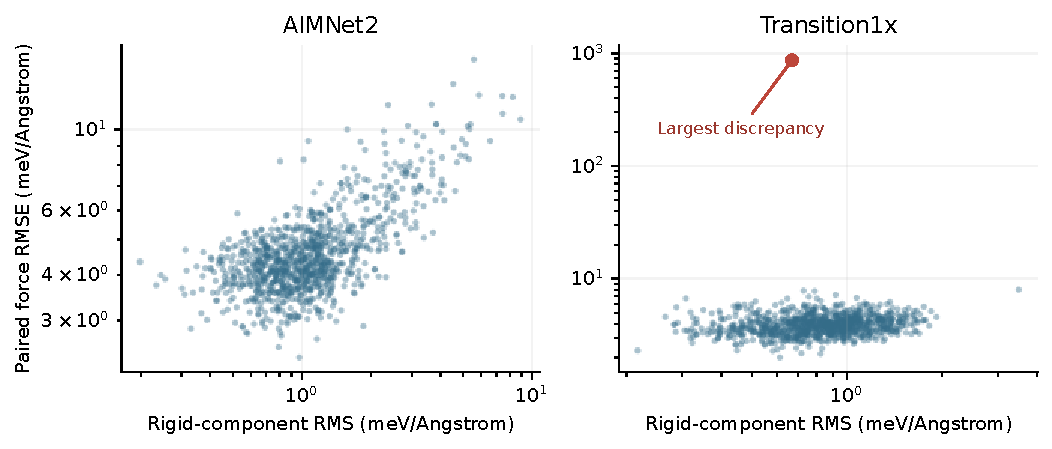
\includegraphics[width=\linewidth]{figures/reliability_scores.pdf}
\caption{Original rigid-component RMS versus paired discrepancy. The Transition1x
record with the largest discrepancy has a modest consistency score. Axes are
logarithmic; each point is a configuration.}
\label{fig:scores}
\end{figure}

\begin{table}[t]
\centering\small\begin{tabular}{lrr}
\toprule
Policy & AIMNet2 (\%) & Transition1x (\%)\\
\midrule
Random, direct & 28.0 [25, 30] & 28.0 [24, 35] \\
Net force, direct & 87.8 [87, 88] & 27.6 [23, 35] \\
Force/torque, direct & 95.0 [95, 95] & 31.8 [30, 35] \\
Force magnitude, direct & 32.8 [32, 35] & 30.6 [24, 38] \\
Geometry novelty, direct & 68.6 [67, 72] & 33.4 [28, 42] \\
Trees, log error & 76.0 [72, 79] & 39.0 [20, 49] \\
Trees, raw error & 76.0 [72, 80] & 36.4 [19, 48] \\
Trees, physical only & 75.6 [71, 80] & 29.2 [18, 39] \\
Ridge & 77.6 [73, 83] & 34.2 [19, 44] \\
MP-pooled ridge & 77.6 [74, 81] & 35.2 [22, 45] \\
\bottomrule
\end{tabular}

\caption{Worst-decile recall at matched total reference counts. Entries are
scenario mean [minimum, maximum] in percent, not confidence intervals. Direct
policies spend the entire budget on selection; learned policies pay seed costs.
The average budget is 28.04\% in each sample.}
\label{tab:recall}
\end{table}

At this budget, direct force/torque screening recovers 95.0\% of the worst decile
on AIMNet2, versus 87.8\% for direct net-force screening and 28.04\% expected under
uniform selection (Table~\ref{tab:recall}). Ridge and MP-pooled ridge both recover
77.6\%, and log-error trees 76.0\%. The learned policies do not improve on the
strongest inexpensive check once seed cost is included.

Cost accounting changes the comparison. If seeds are already available, both
ridge variants recover 77.6\% including seed discoveries, while applying the rigid
score only to the remaining pool recovers 76.0\%. Allowing the direct policy to
spend the complete budget raises its result to 95.0\%. The modest advantage
conditional on existing seeds would be misleading as a claim about a new audit.

On Transition1x, direct force/torque screening recovers 31.8\%, close to the random
expectation of 28.04\%. Log-error trees recover 39.0\%, with a wide range of
20--49\% over scenarios. MP-pooled ridge gives 35.2\% and ordinary ridge 34.2\%.
These finite-sample differences do not establish a universal winner or a
statistically demonstrated RMT advantage.

\begin{figure}[t]
\centering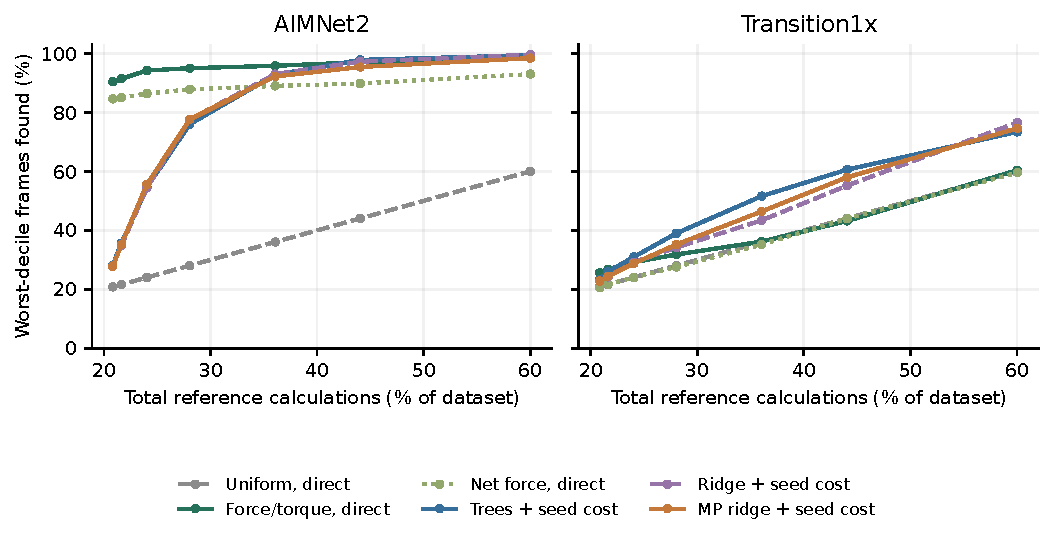
\includegraphics[width=\linewidth]{figures/reliability_budget.pdf}
\caption{Recall versus total reference count. Points average five seed scenarios
at each acquisition fraction. Direct policies receive the same per-scenario total
budget as learned policies, including seed costs. Curves describe overlapping
scenarios rather than independent replications.}
\label{fig:budget}
\end{figure}

\subsection{Detection count and discrepancy impact differ}
The largest Transition1x discrepancy occurs at zero-based file index 255, formula
$\mathrm{C_6H_6O}$. Its frame RMSE is 866.48 meV/\AA, while its net-force score
is 0.3765 and rigid-component RMS 0.6691 meV/\AA. It contributes 97.75\% of total
squared discrepancy. Both direct consistency policies miss it in every primary-
budget scenario. This illustrates Proposition 1; it does not newly identify the
mismatch's electronic cause.

At matched total budgets, net-force and force/torque screening capture only 0.665\%
and 0.675\% of Transition1x squared discrepancy. Ranking by original force magnitude
captures 98.35\%, despite recovering only 30.6\% of the worst decile. Conversely,
log-error trees recover more worst-decile records but capture 39.76\% of squared
discrepancy. Neither endpoint substitutes for the other (Figure~\ref{fig:objectives}).

\begin{figure}[t]
\centering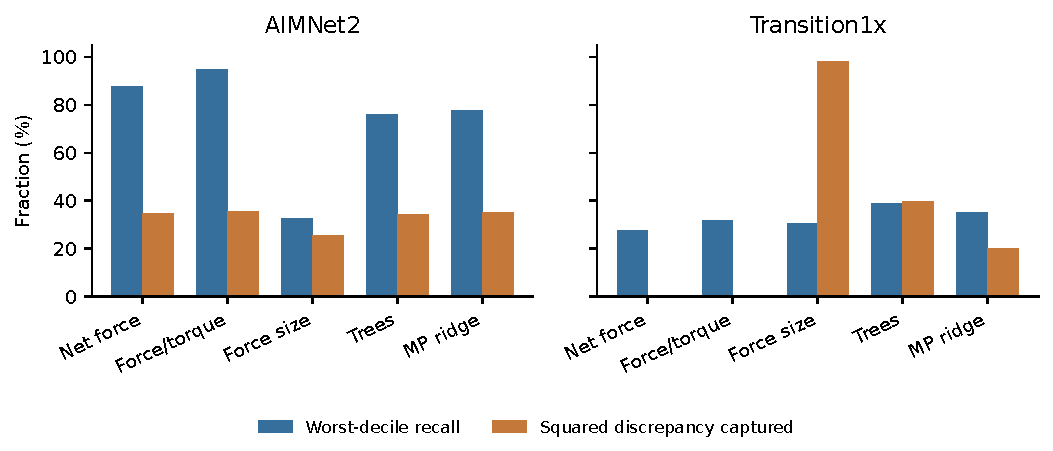
\includegraphics[width=\linewidth]{figures/reliability_objectives.pdf}
\caption{Detection count and squared-discrepancy impact at the primary matched
budget. Transition1x impact is highly sensitive to whether its single large mismatch
is audited. That record is retained in all primary results.}
\label{fig:objectives}
\end{figure}

Fixed tolerances further constrain interpretation. Every primary-budget direct
net-force and rigid-force run recovers all 14 AIMNet2 records above 10 meV/\AA.
In Transition1x the only record above that threshold is the large mismatch: both
direct consistency rules miss it, while force-magnitude ranking finds it. Recall
at 25 meV/\AA\ is undefined for AIMNet2 because no record exceeds the threshold;
the result tables preserve that undefined value.

\subsection{How many references should train the auditor?}
An exploratory extension fixes the total cost at 280 references per 1,000-record
sample. It uses the same five formula folds but draws nested random prefixes of
10, 20, 50 or 100 records from each designated seed fold, alongside the full fold
(mean size 200). Five deterministic permutations are used per fold. The remaining
four folds form a fixed audit pool, independent of prefix size. Unused seed-fold
records are excluded from this pool. All seeds contain at least three formulas;
the original grouped penalty selection and tree settings are retained.

A learned policy uses $m$ references for training and $280-m$ for acquisitions.
Direct policies spend all 280 on the same pool. Only pool discoveries count,
with positives defined as the worst $\lceil0.1|\mathcal U|\rceil$ pool records.
This transfer-to-unseen-formulas endpoint intentionally differs from the earlier
whole-sample recall, which credited seed discoveries. Repeats are averaged within
fold before summarizing the five overlapping scenarios; they are not independent
confirmation datasets. The extension protocol was recorded after examining the
primary results, and no fresh data were introduced.

\begin{figure}[t]
\centering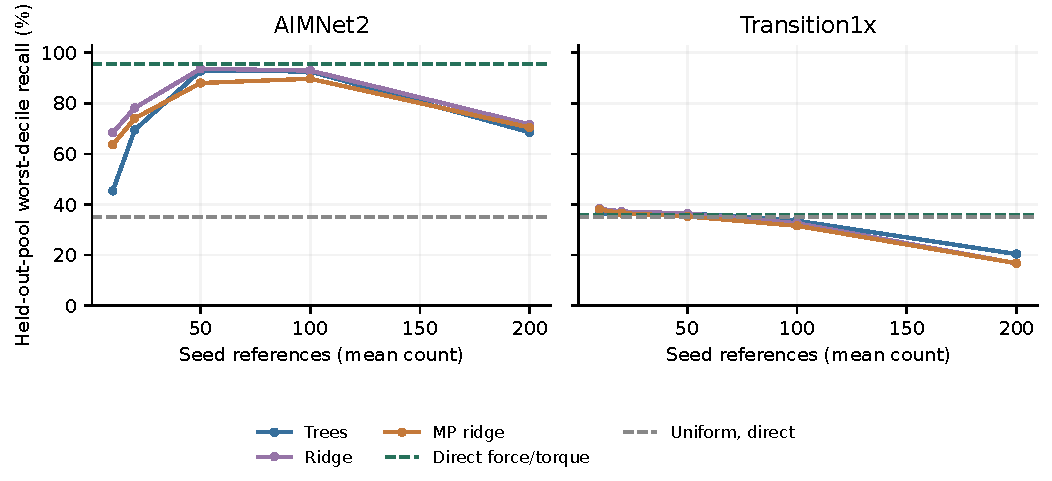
\includegraphics[width=\linewidth]{figures/small_seed_budget.pdf}
\caption{Reference allocation at a fixed total budget of 280. Increasing seed
count leaves fewer acquisitions in the fixed held-out pool. Points average five
seed permutations within each of five formula scenarios. The full-fold point
has mean size 200; its actual size varies by scenario. Direct-policy lines use
280 pool acquisitions throughout.}
\label{fig:smallseed}
\end{figure}

With 50 seed references, log-error trees recover 92.8\%
of the pool's worst decile on AIMNet2 and 36.5\% on
Transition1x. Using the entire seed fold gives 68.5\% and
20.4\%, respectively (Figure~\ref{fig:smallseed}).
At 50 references, ordinary ridge gives 93.7\% and
36.5\%, while MP-pooled ridge gives
88.0\% and 35.3\%.
Direct force/torque screening gives 95.5\% and
36.1\% on these pools.

These curves measure the combined effects of predictor quality and reference
allocation, not prediction error at equal acquisition counts. More training
references need not produce more discoveries under a fixed total budget. The
comparison does not establish a universal optimal seed size, an RMT advantage,
or transfer from these molecular samples to a substantially larger database.


\FloatBarrier
\section{Implications for large computational datasets}
The main finding limits transfer of confidence from a diagnostic that works on one
dataset to another. Consistency checks are inexpensive and reveal some discrepancies
without training references. Yet an audit concentrating only on their violations
can leave large symmetry-compatible discrepancies unchecked. Learned predictors
add information but require reference-budget accounting and seed-sensitivity analysis.

For larger deployment, the proposed workflow retains provenance and solver diagnostics,
runs inexpensive checks across all records, allocates an explicit initial reference
budget, and evaluates complementary acquisition rules on held-out references.
A portion can be reserved for random exploration beyond recognized failure patterns.
The present experiment does not optimize this allocation or validate a hybrid
policy; adding one after these outcomes requires a fresh evaluation protocol.

RMT can be tested for stabilizing correlations or examining repeated-calculation
residuals. Our matrices are descriptor Gram matrices, whose bulk cannot be
interpreted as a direct physical-noise spectrum. A small eigenvalue cannot be
discarded merely because it looks statistically unremarkable. The demonstrated
RMT variant is a comparison component, not a certificate of DFT accuracy.

Several limits govern extrapolation. This is a 2,000-configuration molecular
experiment, not a hundred-thousand-record materials audit. It contains no periodic
stress, magnetic-state or formation-energy ranking benchmark. The primary 20\% average seed budget is substantial. The small-seed extension
tests reference allocation within these samples, but transfer to larger databases
remains untested. Reference counts ignore DFT cost variations with system size
and composition. Pair-distance descriptors cost $O(n_i^2)$ per configuration,
so the implementation does not establish linear scaling to large molecules or solids.

The operational references cannot isolate functional bias or all numerical causes.
The samples also informed earlier exploratory work: the recorded protocol fixes
choices for this audit but does not erase that history. Overlapping scenarios
provide sensitivity analysis rather than independent statistical replication.
Further evidence should use fresh paired data, cost-weighted evaluation and
downstream discovery decisions.

\section{Conclusion}
DFT data reliability can be studied as a budgeted acquisition problem with explicit
reference costs and distinct detection-count and error-impact objectives. Our
paired-data experiment shows strong inexpensive screening on AIMNet2 and a severe
blind spot on Transition1x. Seed costs change the comparison with learned auditors,
while the chosen utility changes which policy looks useful. The results motivate
reporting diagnostic limitations alongside successes. They do not establish
universal noise removal, a special RMT advantage or improved discovery outcomes.

\section*{Data and code availability}
Original paired files are provided by the authors of \citet{kuryla2025} at
\url{https://github.com/water-ice-group/datasets_dft_accuracy}.
The accompanying archive contains the complete analysis, recorded audit protocol,
immutable download manifest, per-scenario predictions and outcomes, and manuscript
source. Original files are downloaded rather than redistributed. Analysis code, results and submission files are available at
\url{https://github.com/SinanGokmen/rmt-reaction-kinetics/tree/main/dft_reliability}.

\section*{Generative AI assistance}
ChatGPT/Codex was used extensively in formulating the research question and
mathematical arguments, implementing and checking code, running the analyses,
searching the literature, and preparing the manuscript and figures. Numerical
results were produced by the accompanying scripts.

\appendix
\section{Reproducibility and supporting checks}
\paragraph{Descriptors and regression.}
Element channels are H, C, N, O, F, S, Cl and other. For each per-atom or pairwise
array we use minimum, 25th percentile, median, 75th percentile, maximum and standard
deviation, followed by $\log(1+x)$. Net, rotational and rigid scores use
$\log(1+s/10^{-3})$ with forces in eV/\AA. Charge is untransformed and atom count
uses $\log(1+n)$. ExtraTrees uses 256 trees, minimum leaf size five, all features
available per split, and random seed $20260911+s$ for scenario $s$. Its physical
ablation uses only net-force and rigid-force inputs. Log targets are
$\log\max(q,10^{-8})$, with $q$ in eV/\AA.

Ridge standardizes nonconstant descriptors using training means and standard
deviations, dividing the Gram matrix by training count. Penalties
$10^{-4},10^{-2},1,100$ are selected by mean log-target squared error in grouped
three-fold validation within seeds. The MP variant replaces eigenvalues below
the nominal edge by their mean before adding the ridge penalty. It is
independently tuned and refitted on all seed references.

\paragraph{Novelty and splits.}
Novelty is squared standardized distance from the whole sample's median in geometry,
composition, charge and atom-count descriptors, excluding force-derived inputs.
Standard deviations use the unlabeled whole sample and are floored at $10^{-8}$.
A formula's fold is the integer represented by the first 12 hexadecimal digits
of SHA-256 of \texttt{dft-denoise-v1:} concatenated with the sorted formula, modulo
five. Ranking ties use increasing original file index. Each primary worst-decile
set contains exactly 100 records.

\paragraph{Unresolved file conventions.}
The available ANI-1x file yields 173.86 meV/\AA\ after the attempted Hartree-to-eV
conversion, rather than the reported comparison. The SPICE file contains 998
frames, a gradient-sign convention and a separate D3 array; the attempted
comparison yields 16.68 meV/\AA. Their correspondence to the published comparisons
remains unresolved. Neither is used in the fitted audit. These checks do not
identify an error in the source publication.

\paragraph{Supporting denoising analysis.}
The earlier pilot, preserved in the archive, projects discrepancies into allowed
and rigid subspaces. The allowed component contains 92.28\% of squared discrepancy
on AIMNet2 and 99.89\% on Transition1x. Element-weighted correction reduced AIMNet2
label RMSE from 4.7979 to 4.4800 meV/\AA\ in its separate grouped protocol. These
are corrected-label results, not the present detection metrics or improved
potential-training results.

\paragraph{Verification.}
Changing tight forces and energies while holding original results fixed changes
no input feature. Rigid coordinate transformations change descriptors by at most
$5.63\times10^{-14}$ on checked configurations. Saved predictions never pair a
target with its seed formula fold. Primary recalls reconstructed from saved scores
match exactly, and acquisition sets have the specified distinct-record counts.
The archive includes 80,000 scenario-method score rows and 4,760 metric rows for
2,000 unique configurations; those rows are not additional independent samples. The small-seed extension
adds 250 seed sets, 1,000,000 score rows and 2,250 metric rows on the same
configurations. Independently reconstructing its acquisition sets and metrics
agrees to within $1.12\times10^{-16}$; all nested-seed and formula-separation
checks pass.

\clearpage
\bibliographystyle{plainnat}
\bibliography{references}
\end{document}
